% Created 2017-04-20 Thu 14:50
% Intended LaTeX compiler: xelatex
\documentclass[a4paper, notitlepage]{report}
\usepackage{graphicx}
\usepackage{grffile}
\usepackage{longtable}
\usepackage{wrapfig}
\usepackage{rotating}
\usepackage[normalem]{ulem}
\usepackage{amsmath}
\usepackage{textcomp}
\usepackage{amssymb}
\usepackage{capt-of}
\usepackage{hyperref}
% set the margins here, if they need to be modified
\usepackage[a4paper, left=1.3in, right=1.0in]{geometry}

\usepackage[style=ieee,backend=biber]{biblatex}

% The linespacing you want
\linespread{1.4}

% Lets you pick fonts. Only works if you compile with xelatex or luatex
\usepackage[no-math]{fontspec}

\usepackage{unicode-math}

\usepackage{stackengine}
\stackMath

% Used to make the captions on figures sans serif
\usepackage{caption}

% For including images
\usepackage{graphicx}
\usepackage{float}

\usepackage{color}

% For fancy code listings
\usepackage{minted}
\usemintedstyle{emacs}

% For tables that span multiple pages elegantly
\usepackage{longtable}

% For maintaining a list of abbreviations
\usepackage{nomencl}

% For drawing diagrams
\usepackage{tikz}

% These closely match the SCSS word template fonts
% Won't work unless you compile with xelatex or luatex
\setmainfont[Mapping=tex-text]{Times New Roman}
\setsansfont{Helvetica}
\setmonofont[Scale=MatchLowercase]{Monaco}
\setmathfont{TeX Gyre Termes Math}

\hypersetup{
  colorlinks,
  citecolor=black,
  filecolor=black,
  linkcolor=black,
  urlcolor=black
}

% Change these as appropriate, and they'll be filled in automatically on the
% cover page. You can also use them throughout the document, so as not to have
% to type them again all the time.
\newcommand \authorname{Eoin Houlihan}
\newcommand \authoremail{ehoulih@tcd.ie}
\newcommand \supervisorname{Dr. Glenn Strong}
\newcommand \degreetitle{B.A.(Mod.) Computer Science}
\newcommand \projecttitle{Dependent Types in Practice}

% All the commands are defined in this file
\newcommand \inserttitlepage{\thispagestyle{empty}
\begin{center}
{\sffamily
{\Large University of Dublin}

\vspace{10pt}


\includegraphics[scale=0.12]{tcd/trinitycollege.pdf}

\vspace{10pt}

{\Huge TRINITY COLLEGE}

\vspace{80pt}

\textbf{ \Large \emph \projecttitle}

\vspace{30pt}

\authorname

\degreetitle

Final Year Project May 2017

Supervisor: \supervisorname

\vspace{130pt}

\large{School of Computer Science and Statistics
\\$ $\\
O'Reilly Institute, Trinity College, Dublin 2, Ireland}
\linespread{1}
}
\end{center}
}
\newcommand \insertabstract{\begin{abstract}
\thispagestyle{plain}
Major software vulnerabilities in critical software have led to more interest in
formal verification of our software. One way that has presented itself to verify
our code is by using dependent types, an idea from the 1970s present in a number
of upcoming programming languages and interactive theorem provers.

We present a study into the current state-of-the-art dependently-typed
programming languages. Idris was chosen as the tool to carry out this study. The
methodology involved carrying out case studies of applying dependent types to
real-world programming problems. An evaluation of the outcomes and the current
landscape of dependently-typed programming languages applied in a practical
sense is provided as a result of carrying out these case studies.
\end{abstract}
}
\newcommand \declaration{\chapter*{Declaration}

I hereby declare that this project is entirely my own work and that it has not
been submitted as an exercise for a degree at this or any other university.
$ $\\
$ $\\
\signed{\authorname}
}
\newcommand \acknowledgements{\chapter*{Acknowledgements}
Firstly, I would like to thank my parents for giving me the opportunity, support
and encouragement I needed throughout my degree.

\noindent
I would like to thank Glenn Strong for his continued guidance and suggestions
throughout this project as my supervisor.

\noindent
I would also like to thank the budding Idris and dependent type community,
particularly those in the \#idris IRC channel, for being patient enough to
answer any questions that I had.
}
\newcommand \permissiontolend{\chapter*{Permission to lend}

I agree that the Library and other agents of the College may lend or copy
this report upon request.

$ $\\
$ $\\
\signed{\authorname}
}
\newcommand \ibidp{(\emph{Ibid.})}
\newcommand \ibid{\emph{Ibid.}}

\newcommand{\argmax}[1]{\underset{#1}{\operatorname{arg}\,\operatorname{max}}\;}

\usepackage{datetime}

\def\fullhrulefill{\leavevmode\leaders\hrule height 1pt\hfill\kern 0pt}

\newcommand{\signedanddate} {
  \par\noindent\makebox[2.5in]{\fullhrulefill}
  \par\noindent\makebox[2.5in][l]{\authorname, May 5 2017}
}

\newcommand \needcite[1]{\underline{#1}}

\newcommand \abbrev[2]{#1\nomenclature{#1}{#2}}


% For changing the names of the List of Listings, etc.
\renewcommand*{\contentsname}{Table of Contents}
\renewcommand*{\nomname}{Abbreviations}

% Make the captions sans serif
\renewcommand{\captionfont}{\sffamily}

\addbibresource{report.bib}
\usepackage{draftwatermark}
\SetWatermarkLightness{0.95}
\author{Eoin Houlihan}
\date{\today}
\title{}
\hypersetup{
 pdfauthor={Eoin Houlihan},
 pdftitle={},
 pdfkeywords={},
 pdfsubject={},
 pdfcreator={Emacs 25.2.1 (Org mode 9.0.5)},
 pdflang={English}}
\begin{document}

\inserttitlepage
\pagenumbering{roman}
\declaration
\permissiontolend
\insertabstract
\acknowledgements
\tableofcontents
\newpage
\pagenumbering{arabic}

\chapter{Introduction}
\label{sec:orge810b24}
\chapter{Background}
\label{sec:orgd9b1c6a}
This chapter aims to give an understanding of the background and necessary
concepts that will be used throughout the report. A basic understanding of
functional programming ideas such as algebraic data types, recursion and the
fundamentals of the Hindley-Milner type system with respect to languages such as
Haskell is assumed of the reader. It also gives a broad overview of the current
state of the art dependently-typed programming languages with a more in-depth
look at Idris in particular.

\section{Intuitionistic Type Theory}
\label{sec:org3f7e140}
Intuitionistic type theory is a type theory based on mathematical
constructivism. Constructive mathematics is an alternative foundational theory
of mathematics that argues that construction of a mathematical object is
necessary to proving that such an object exists. Of particular note, the
intuitionistic logic which much of constructivism uses deviates from classical
logic systems in that proof by contradiction is not used and the law of the
excluded middle is not assumed as an axiom of the logic in general.

Drawing upon these ideas, Per Martin-Löf, a Swedish logician, developed a number
of successive type theories in the 1970s \cite{martin-lof_intuitionistic_1984}.
This intuitionistic type theory (also commonly referred to as Martin-Löf type
theory) introduces a number of interesting concepts. Most notable in terms of
their influences on programming language design were the concepts of \(\Pi\)-types
and \(\Sigma\)-types. These constructs can be seen as analogous to the logical
quantifiers ``forall'' and ``exists'' respectively. These concepts have served
as the underpinning of the development of dependently-typed programming
languages and theorem provers based on Martin-Löf type theory.

\section{Curry-Howard Isomorphism}
\label{sec:org6829dd0}
From a modern computer science perspective it's almost taken for granted that
computability theory and mathematical proofs are inherently linked. For example,
many parallels can be drawn between the proof of Turing's Halting Problem and
Gödel's incompleteness theorems. Between the 1930s and the 1960s Haskell Curry
and William Alvin Howard began to formalise this direct link between computer
programs and mathematical proofs which is known as the Curry-Howard isomorphism
\cite{mcadams_tutor_2013}. As Philip Wadler, one of the original authors of the
Haskell report, put it \cite{strange_loop_2015,wadler_propos_2015}

\begin{quote}
``Every good idea will be discovered twice. Once by a logician and once by a
computer scientist'' -- Philip Wadler
\end{quote}

According to the Curry-Howard isomorphism the type of an expression is
equivalent to a proposition of a logical formula. A term inhabiting that type is
therefore equivalent to a proof that the proposition holds. Some concrete value
exists that bears witness to the type being inhabited. In other words, a proof
can be constructed. This very much aligns with the constructivist view of
mathematics. Other correspondences can be shown such as between logical
implication and function types, conjunction and product types and between false
formulas and the uninhabited type, bottom (\(\bot\)). We can even see from the
shape of the syntax rules of both natural deduction and simply-typed lambda
calculus that these kinds of correspondences exist. As an example, the
relationship between the Modus Ponens rule and the function application rule.
\[ \scalebox{2}{$\frac{\Gamma \vdash \alpha \rightarrow \beta \qquad \Gamma
\vdash \alpha}{\Gamma \vdash \beta} \rightarrow E \qquad \frac{\Gamma \vdash
t:\alpha \rightarrow \beta \qquad \Gamma \vdash u:\alpha}{\Gamma \vdash
t\;u:\beta}$} \]

One of the consequences of this relationship is the possibility of a unification
at a primitive level between mathematical logic and the foundations of
computation. In practical terms this relationship has influenced the work on
programming languages such as Coq and Idris that allow proofs to be written as
programs that can be formalised, verified and executed. This is interesting to
the practice of software engineering as it gives us the power to reason about
program correctness by translating a mathematical proof of an algorithm to a
computer program and having the machine type-check (proof-check) it.

\section{Traditional Hindley-Milner Type Systems}
\label{sec:orgfdcdf0c}
Standard Hindley-Milner-esque type systems such as the one found in Haskell
allow us to express some different dependencies between the types of terms and
terms themselves. For example, terms can depend on other terms such as in this
Haskell function definition.

\begin{minted}[frame=single,fontsize=\scriptsize,linenos,escapeinside=\#\#]{haskell}
plusOne x = x + 1
\end{minted}

Here we can see that the term \texttt{plusOne} has been defined with respect to the
terms \texttt{x}, which is its argument and \texttt{1}, an integer. Types can also depend on
other types as shown here.

\begin{minted}[frame=single,fontsize=\scriptsize,linenos,escapeinside=\#\#]{haskell}
data List a = Nil
            | Cons a (List a)
\end{minted}

In this Haskell data type definition, the type constructor \texttt{List} depends on the
type \texttt{a} provided to it. This allows polymorphism and lists of any type.
Finally, in the world of Haskell, terms can depend on types. This is apparent in
polymorphic functions such as the identity function.

\begin{minted}[frame=single,fontsize=\scriptsize,linenos,escapeinside=\#\#]{haskell}
id :: a -> a
id x = x
\end{minted}

\section{Dependent Type Systems}
\label{sec:org4711820}
Dependent type systems extend this system of dependencies by allowing types to
depend on terms. This leads to much greater expressivity power in the type
system. For example, in a dependently typed system we can express types such as
the type of pairs of natural numbers where the second number is greater than the
first.

If we take the view of the Curry-Howard isomorphism that types are propositions
and terms are witnesses to a proof of that proposition then we can see the
advantages of a more expressive type system. We can now encode much more
sophisticated propositions in the type system and if we can prove them (i.e.
construct a value that inhabits that type) then we can guarantee much more
interesting correctness properties about the code that we are writing. For this
reason, dependent types have seen much use in the areas of formal verification
of computer programs and formal computer encoding of mathematical objects and
proofs.

There are 3 main concepts taken from Martin-Löf type theory and implemented in
dependently-typed programming languages.

\subsection{\texorpdfstring{$\Pi$}{Pi}-types}
\label{sec:org5d0b81c}
\(\Pi\)-types are the types of functions whose return types depend on one or more of
their arguments. In other words these functions map values from some domain to
some non-fixed codomain that is determined by the input. In this sense the
return type is said to be dependent upon the input.

If we have a representation of \(n\textrm{-tuples}\) of some type \(A\),
\(\operatorname{Vect}(A,n)\), then the \(\Pi\)-type \(\Pi_{(n \mathbin{:} {\mathbb N})}
\operatorname{Vect}(A,n)\) represents the type of functions that given some
natural number \(n\) return a tuple of size \(n\) of elements of type \(A\). That is
to say that the type of the value returned by these functions is determined by
the argument to the functions.

\subsection{\texorpdfstring{$\Sigma$}{Sigma}-types}
\label{sec:org0bda34b}
\(\Sigma\)-types, also known as dependent pair types, are a more generalised form of
Cartesian product that model pairs of values where the type of the second
element depends on the first element.

Again using the \(\operatorname{Vect}\) representation of \(n\textrm{-tuples}\) of
some type \(A\), the \(\Sigma\)-type \(\Sigma_{(n \mathbin{:} {\mathbb N})}
\operatorname{Vect}(A,n)\) represents a pair of a natural number \(n\) and a tuple
of length \(n\) of values of type \(A\).

This representation is similar to the Haskell \texttt{List} type however there is extra
information in that the type of the \(\Sigma\)-type \(\operatorname{Vect}\) also
carries around a witness to its length expressed as a natural number. We say
that \(\operatorname{Vect}\) is ``indexed'' by the type \(A\) as well as the value
\(n\).

Being able to index types by both types and terms in the language is a key
feature of dependently-typed programming languages. These languages eliminate
the distinction between types and terms. Types and terms are unified as
equivalent constructs.

\subsection{The Equality Type}
\label{sec:org8b5af8c}
The equality type \(=\) is a special type used to denote proofs of equality
between two values. If there is an inhabitant of the type \(a \mathrel{=} b\) then
\(a\) and \(b\) are considered to be equal. This proof allows \(b\) to be used
anywhere \(a\) would have been used. There is only one inhabitant of the type \(a
\mathrel{=} a\), the reflexive proof of equality.

\[ \scalebox{2}{$\operatorname{refl} \mathbin{:} \Pi_{(a \mathbin{:} A)} (a
\mathrel{=} a)$} \]

This type is particularly useful in dependently-typed programming in that it can
be used as a witness that two terms are equivalent and allows a substitution of
one term for another to take place. With it, we can begin to develop
constructions of basic proofs and axioms such as \(n \mathbin{:} {\mathbb N}, n
\mathbin{-} n \mathrel{=} 0\).

\section{State of The Art Dependently-Typed Programming Languages}
\label{sec:org06358d1}
\subsection{Agda}
\label{sec:org7ea3266}
Originally developed in the late 1990s by Catarina Coquand and subsequently
rewritten by Ulf Norell in 2007, Agda is a dependently typed programming
language with support for features such as dependent pattern matching and
definition of inductive data types.

For example, the inductive data type representing the Peano natural numbers can
be declared as follows in Agda.

\begin{minted}[frame=single,fontsize=\scriptsize,linenos,escapeinside=\#\#]{agda}
data #$ℕ$# : Set where
  zero : #$ℕ$#
  suc : #$ℕ$# → #$ℕ$#
\end{minted}

There are two cases to consider here. \texttt{zero} is the base case. \texttt{suc} (standing
for successor) takes a natural number and returns a new natural number. It
represents a natural number plus 1. We will see more definitions of inductive
types similar to this one throughout the later chapters.

Agda has the capability of producing executable code however it is mostly used
for the purpose of automated theorem proving. Agda does however provide a
foreign function interface to import arbitrary Haskell types and functions.
These go unused for the purpose of Agda type-checking but do have runtime
effects in the output compiled code.

\subsection{Coq}
\label{sec:org1999dab}
Developed initially in the late 1980s at INRIA in France, Coq approaches
dependently-typed programming more from the mathematical side as an interactive
theorem prover. Coq is based on the Calculus of Constructions, a type theory
created by Thierry Coquand. Coq provides useful facilities for defining
inductive data types and includes a tactics language for doing interactive
proofs.

Notable work created using Coq includes the formally verified C compiler
CompCert \cite{compcert}, as well as a formally verified proof of the Four-Colour
Theorem \cite{gonthier_formal_2008} for graph colouring.

Development in Coq and using dependent types in general can become quite
complex. To support the powerful type system a number of featureful interactive
environments such as CoqIDE and Proof General \cite{proof_general} exist. These
environments provide semantic information about your code. This includes the
current environment of defined values as well as their types and the type of the
current goal that you are attempting to prove.

\begin{figure}[H]
\centering
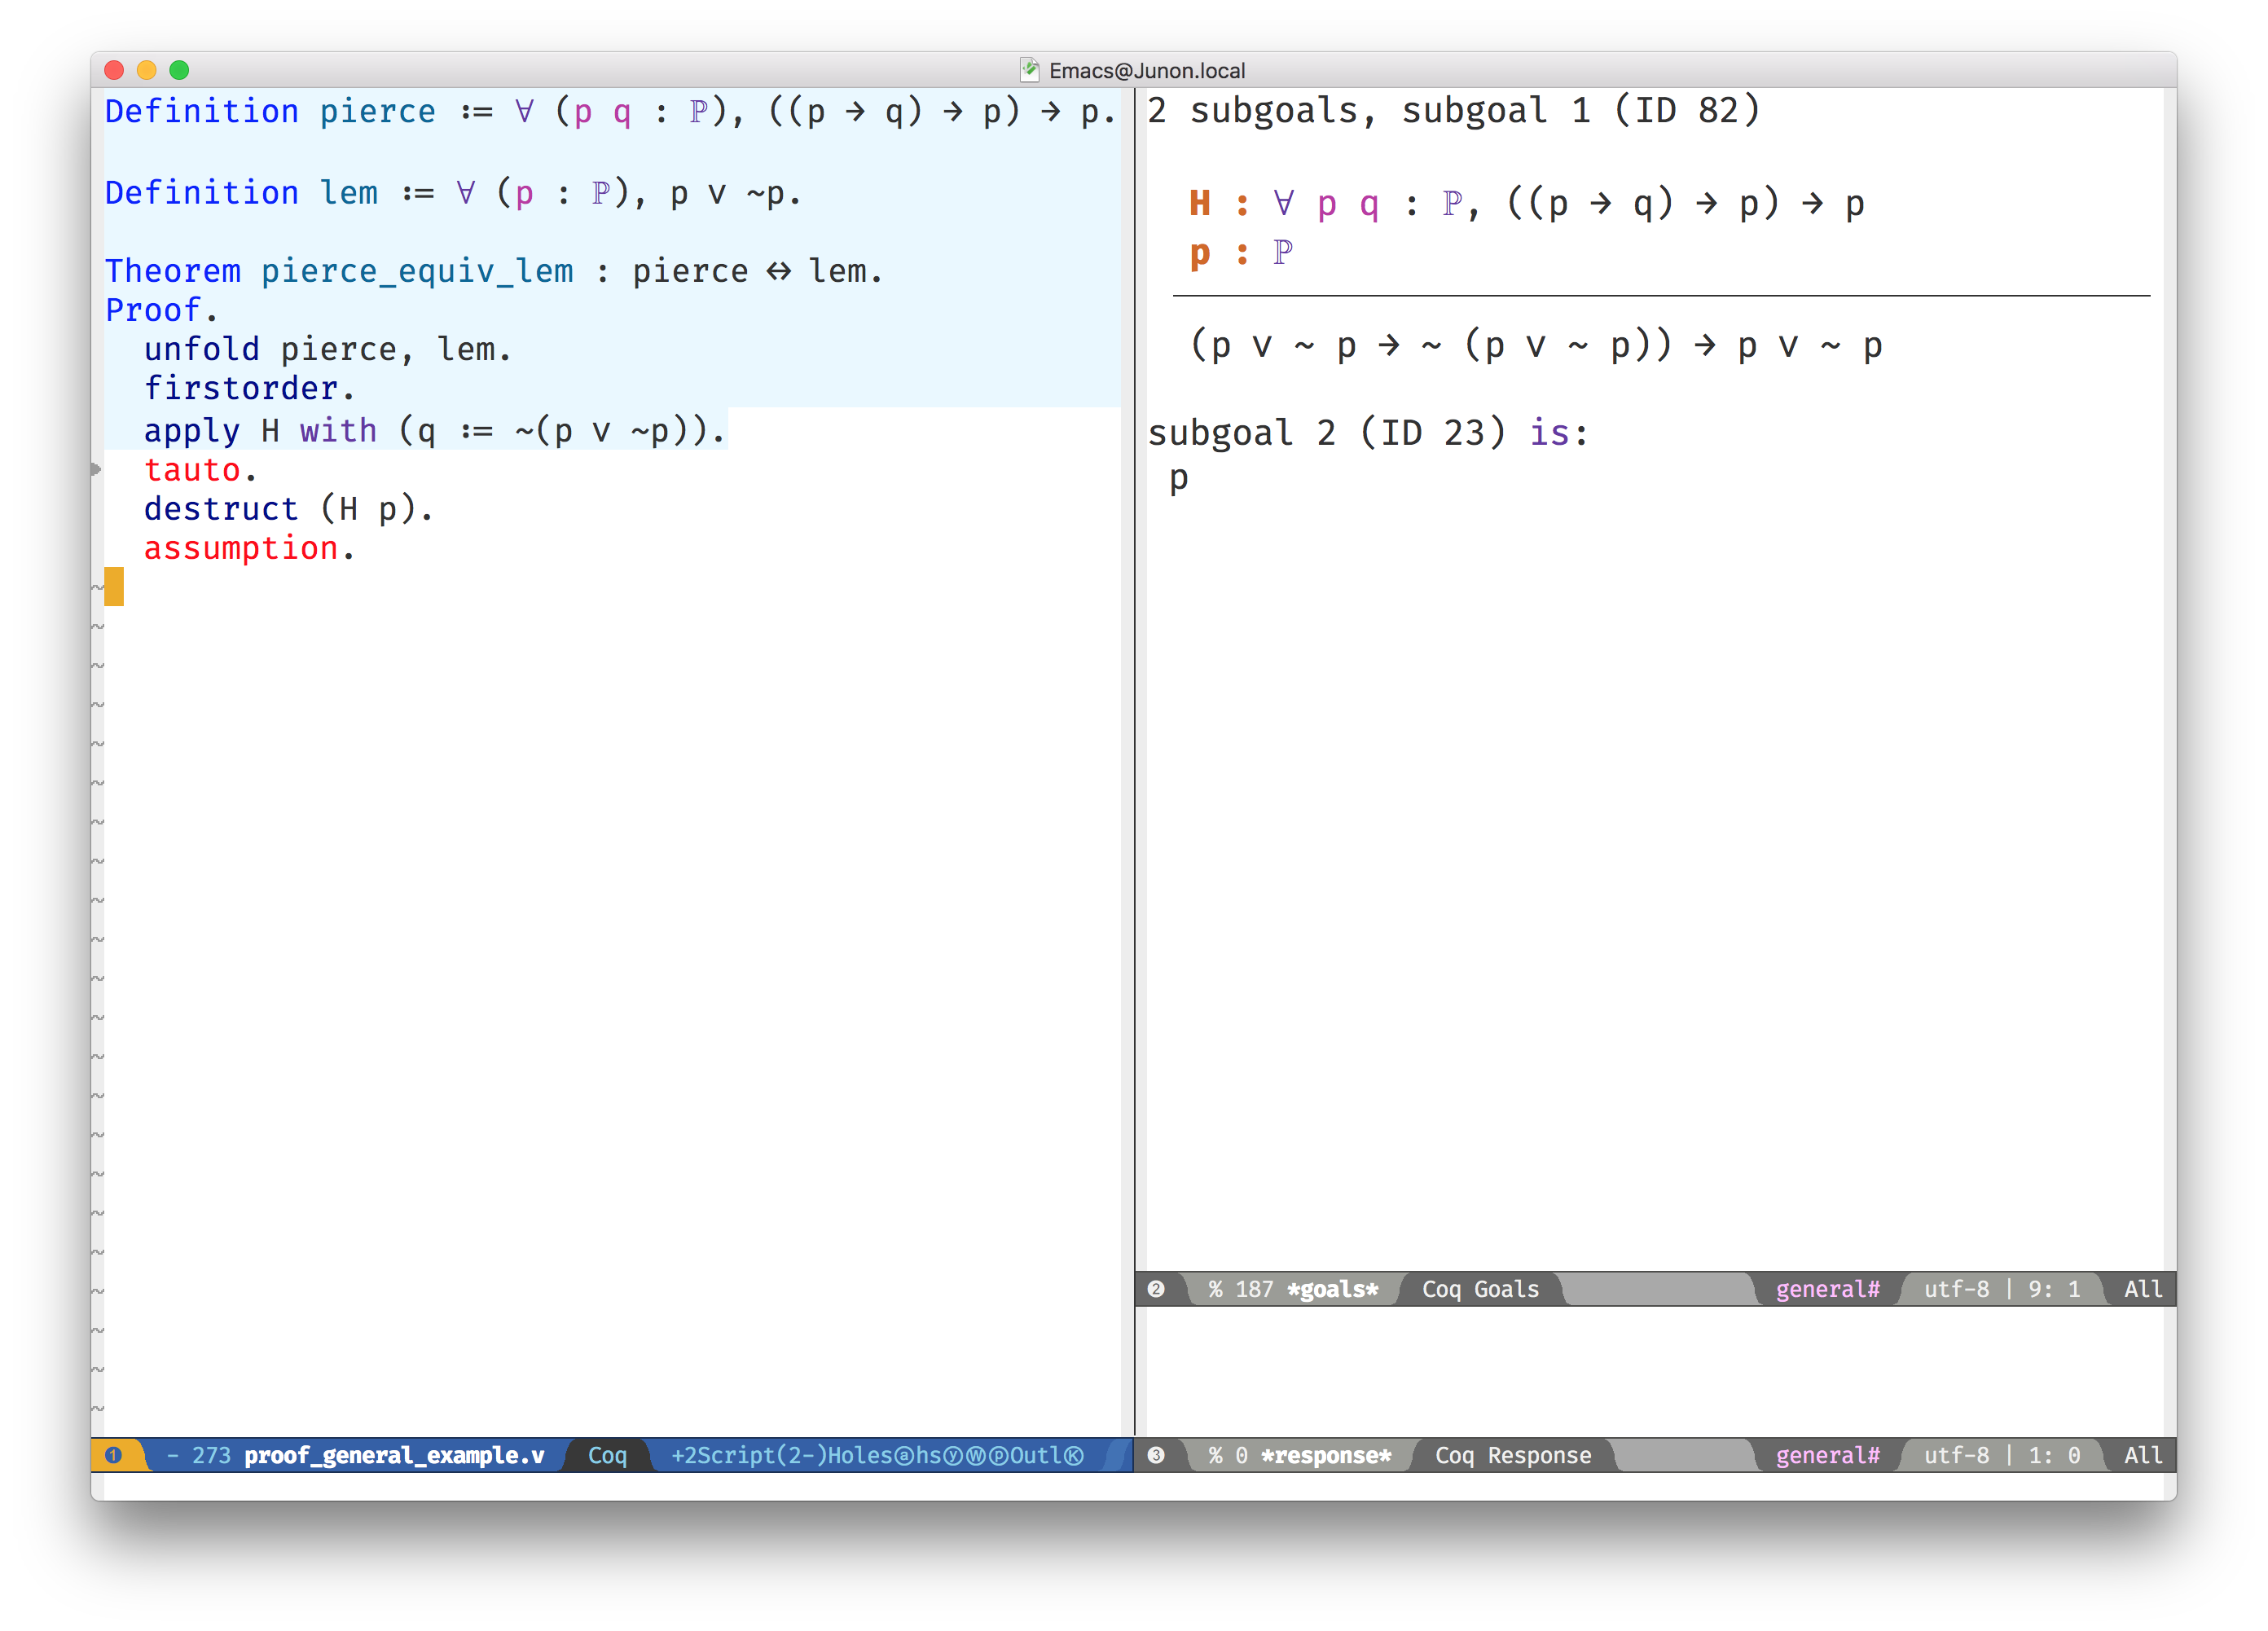
\includegraphics[width=0.85\linewidth]{./fig/proof_general.png}
\caption{An in-progress Proof General session}
\end{figure}

Coq's primary mechanism for producing executable code is via program extraction.
This is the process by which correct Coq code can be transformed into an
equivalent Haskell or OCaml module which provides the user with the ability to
run the extracted code. This extraction process has benefits in that it allows
for the expression and type-checking of interesting correctness properties in a
dependently-typed language while also giving us a way to compile it to native
code using compilers with state-of-the-art code optimisation techniques. This
allows the production of a fast native binary from a correct and type-checked
Coq program.

\subsection{Haskell}
\label{sec:org375ef18}
GHC Haskell has slowly been implementing many of the capabilities of dependent
types via extensions to the language such as \texttt{GADTs}, \texttt{DataKinds}, and
\texttt{TypeFamilies}. Through particular use of the Haskell type system many of the
features of dependently typed languages can be simulated in roundabout ways
\cite{mcbride_faking_2002,lindley_hasochism_2013}.

A full dependent type system is currently being implemented for future releases
of GHC 8 \cite{eisenberg_dependent_2016,weirich_specif_2017}. Existing
extensions and offshoots of GHC such as Liquid Haskell implement refinement
types which allows for the expression of a limited set of propositions at the
type level in existing Haskell code \cite{vazou_refinement_2014}.

\subsection{Idris}
\label{sec:orga208819}
Idris is primarily the work of Edwin Brady and others at the University of St.
Andrews in Scotland. It has positioned itself as a more practical take on
dependently-typed programming and as such is more aimed at being a language that
you can write programs leveraging dependent types while also performing
interesting effectful actions such as file I/O and drawing graphics to the
screen.

Edwin Brady, the author of Idris has said before that Idris has the interesting
property of being ``Pac-Man Complete'' \cite{scala_world_2015}. Rather than just
being a Turing complete language, if you wanted to, you could write a version of
a simple 2D game such as Pac-Man in the language.

This report focuses on using Idris in a practical manner while aiming to take
advantage of dependent types to ensure that our code is more correct.

\section{The Idris Programming Language}
\label{sec:orgc5902f7}
\subsection{Similarities to Haskell}
\label{sec:org7f58cdc}
Idris has inherited much of the surface syntax of Haskell and will be quite
familiar to anyone who has worked in Haskell or a similar ML-like language
before. For example, the function that calculates the length of the list would
look as follows in Haskell.

\begin{minted}[frame=single,fontsize=\scriptsize,linenos,escapeinside=\#\#]{haskell}
length :: [a] -> Integer
length [] = 0
length (_:xs) = 1 + length xs
\end{minted}

An equivalent Idris function bears some resemblance with notable exceptions
being the explicit name \texttt{List} as the list type constructor and the swapping of
the type operator (\texttt{::}) and the cons operator (\texttt{:}).

\begin{minted}[frame=single,fontsize=\scriptsize,linenos,escapeinside=\#\#]{idris}
length : List a -> Integer
length [] = 0
length (_::xs) = 1 + length xs
\end{minted}

Data-type declarations also follow a similar syntax with Idris code favouring
the explicit type signature style seen in Haskell GADTs. As an example we could
have a simple data type such as a list implemented in Haskell.

\begin{minted}[frame=single,fontsize=\scriptsize,linenos,escapeinside=\#\#]{haskell}
data List a = Nil
            | Cons a (List a)
\end{minted}

In Idris we could define it the same way however the idiom is to use the
explicit type signatures as it becomes the only way to implement more powerful
dependently-typed data types later on.

\begin{minted}[frame=single,fontsize=\scriptsize,linenos,escapeinside=\#\#]{idris}
data List : Type -> Type where
  Nil : List a
  Cons : a -> List a -> List a
\end{minted}

\subsection{Typed Holes}
\label{sec:org698881d}

\subsection{Implicit Arguments}
\label{sec:org5cbec9c}

\subsection{Total Functional Programming}
\label{sec:orgb902d5a}
One of the key concepts advocated by the language designers of Idris is the
concept of ``total'' functional programming. From languages such as Haskell you
may be familiar with functions such as \texttt{head} and \texttt{tail} on lists which have the
possibility of crashing at runtime.

\begin{minted}[frame=single,fontsize=\scriptsize,linenos,escapeinside=\#\#]{idris}
head : List a -> a
head (x::_) = x

tail : List a -> List a
tail (_::xs) = xs
\end{minted}

Both of these functions will crash our programs at runtime if we call them with
the empty list but will still pass Idris' type checker. The reason for this is
that the functions are partial. Both functions fail to provide a function clause
that will match the empty list as an input resulting in a runtime error but not
a type error. The simple solution to this is define some safe versions of these
functions using the \texttt{Maybe} type.

\begin{minted}[frame=single,fontsize=\scriptsize,linenos,escapeinside=\#\#]{idris}
head : List a -> Maybe a
head [] = Nothing
head (x::_) = Just x

tail : List a -> Maybe (List a)
tail [] = Nothing
tail (_::xs) = Just xs
\end{minted}

We now have total versions of these functions in so far as they guarantee to
always return a result for any well-typed input. This style of ``total''
functional programming is heavily recommended in Idris. In fact, any function
that we use to compute a type must pass the compiler's built-in totality
checker. If the function is not total it leaves us with the possibility of a
runtime error in the type checker when computing the value of the function.

Functions that do not terminate are also partial functions in that they can
never produce a result. If these functions were total we could have a type that
could never be computed to some normal form and cause the Idris type checker to
run forever.

\begin{minted}[frame=single,fontsize=\scriptsize,linenos,escapeinside=\#\#]{idris}
loop : a -> b
loop x = loop x
\end{minted}

To think about functions in terms of proofs leaves us with some interesting
implications for totality. A partial function can only guarantee us that when it
is provided inputs of the correct type it will produce a proof if it terminates.
A total function on the other hand gives us a much stronger guarantee that if
the function is provided inputs of the correct type it will terminate and it
will produce the proof (the value). When dealing with functions that compute
proofs it is quite important that we ensure that our definitions are total to be
confident that our proof holds in all cases. A partial program that just
infinitely loops will satisfy any type that we give it.

Idris provides some mechanisms to help prevent us from writing partial code. The
first of which is the \texttt{total} annotation. We can add this to any function
definition and the effect is that the compiler enforces that the function is
indeed total. Failure to pass the Idris totality checker results in a message
from the compiler. Trying out the bad \texttt{loop} code from above with the \texttt{total}
annotation added results in the Idris compiler informing us that our definition
is not total due to the recursion in our function clause.

\begin{minted}[frame=single,fontsize=\scriptsize,linenos,escapeinside=\#\#]{idris}
total
loop : a -> b
loop x = loop x
-- When loaded: Main.loop is possibly not total due to recursive path Main.loop --> Main.loop
\end{minted}

The second mechanism is mainly a convenience for the first. If we include the
compiler pragma \texttt{\%default total} at the top of our Idris module, all definitions
after it will be checked for totality. The \texttt{partial} annotation can then be used
as an escape hatch from the totality checker. When working on code we would like
to prove not only for correctness but for totality it makes sense to begin all
of our modules with this compiler pragma and use the \texttt{partial} annotation where
necessary. This pragma is used throughout the code outlined in the case studies
in the later chapters.
\chapter{My Project}
\label{sec:org5c9b282}

\section{Objectives}
\label{sec:org4f05fc6}

\section{Approach}
\label{sec:orgcd48381}

\section{Type-Driven-Development}
\label{sec:orgca246b2}

\section{Interactive Editing Modes for Idris}
\label{sec:org5e87485}
\chapter{Case Studies}
\label{sec:orgeddb02d}
\chapter{Assessments and Conclusions}
\label{sec:org91f2472}
\chapter{Future Work}
\label{sec:org889d519}

\emergencystretch=1em
\printbibliography
\appendix
\end{document}